\chapter{In Depth: Principal Component Analysis\label{Ch45}}

\section{Introducing Principal Component Analysis}
These vectors represent the principal axes of the data, and the length of each vector is
an indication of how “important” that axis is in describing the distribution of the data
—more precisely, it is a measure of the variance of the data when projected onto that
axis. The projection of each data point onto the principal axes are the principal components of the data.

This transformation from data axes to principal axes is an \textbf{affine transformation},
which means it is composed of a translation, rotation, and uniform scaling.

\subsection{PCA as Dimensionality Reduction}
Using PCA for dimensionality reduction involves zeroing out one or more of the
smallest principal components, resulting in a lower-dimensional projection of the
data that preserves the maximal data variance.

\subsection{What Do the Components Mean?}
We can go a bit further here, and begin to ask what the reduced dimensions mean.
This meaning can be understood in terms of combinations of basis vectors.
\subsection{Choosing the Number of Components}
A vital part of using PCA in practice is the ability to estimate how many components are needed to describe the data. This can be determined by looking at the cumulative \textbf{explained variance ratio} as a function of the number of components.

\begin{figure}
    \centering
    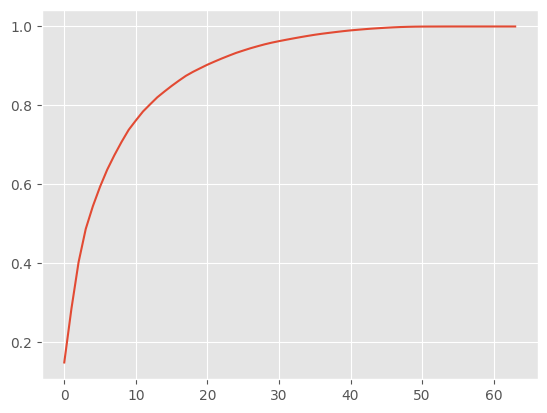
\includegraphics{../Figures/fig45-8.png}
    \caption{The cumulative explained variance, which measures how well PCA preserves the content of the data}
\end{figure}

This tells us that our two-dimensional projection loses a lot of information (as measured by the explained variance) and that we'd need about 20 components to retain
90\% of the variance. Looking at this plot for a high-dimensional dataset can help you
understand the level of redundancy present in its features.

\section{PCA as Noise Filtering}
PCA can also be used as a filtering approach for noisy data. The idea is this: any components with variance much larger than the effect of the noise should be relatively unaffected by the noise. So, if you reconstruct the data using just the largest subset of principal components, you should be preferentially keeping the signal and throwing out the noise.

\section{Example: Eigenfaces}
In this case, it can be interesting to visualize the images associated with the first several principal components (these components are technically known as \textbf{eigenvectors}, so these types of images are often called \textbf{eigenfaces}; as you can see in \autoref{A visualization of eigenfaces learned from the LFW dataset}, they are as creepy as they sound)
\figures{A visualization of eigenfaces learned from the LFW dataset}

The results are very interesting, and give us insight into how the images vary: for example, the first few eigenfaces (from the top left) seem to be associated with the angle of lighting on the face, and later principal vectors seem to be picking out certain features, such as eyes, noses, and lips.

\section{Summary}

Given any high-dimensional dataset, I tend to start with PCA in order to visualize the relationships between points (as we did with the digits data), to understand the main variance in the data (as we did with the eigenfaces), and to understand the intrinsic dimensionality (by plotting the explained variance ratio). Certainly PCA is not useful for every high-dimensional dataset, but it offers a straightforward and efficient path to gaining insight into high-dimensional data.

\important{PCA's main weakness is that it tends to be highly affected by outliers in the data.} For this reason, several robust variants of PCA have been developed, many of which act to iteratively discard data points that are poorly described by the initial components.